\documentclass[10pt,a4paper]{article}
\usepackage[margin=0.9in]{geometry}
\usepackage[T1]{fontenc}
\usepackage{lmodern}
\usepackage{microtype}
\usepackage{amsmath,amssymb,booktabs,graphicx}
\usepackage[numbers,sort&compress]{natbib}
\usepackage{xcolor}
\usepackage[hidelinks]{hyperref}
\usepackage{url}
\newcommand{\BenchEntries}{2,579}
\newcommand{\LegacyEntries}{2,164}
\newcommand{\SunoEntries}{200}
\newcommand{\UdioEntries}{200}
\newcommand{\LyriaEntries}{11}
\newcommand{\StableAudioEntries}{4}
\newcommand{\RecordingGroups}{2,576}
\newcommand{\DependenceClusters}{2,456}
\newcommand{\NativePairs}{3}

\newcommand{\CheckpointLegacyFone}{0.9887}
\newcommand{\CheckpointMixedFone}{0.9327}
\newcommand{\CheckpointSunoRawTpr}{5.0}
\newcommand{\CheckpointSunoRawLow}{1.9}
\newcommand{\CheckpointSunoRawHigh}{8.9}
\newcommand{\CheckpointSunoStackTpr}{7.5}
\newcommand{\CheckpointLyriaTP}{0}
\newcommand{\CheckpointStableTP}{0}

\title{ArtifactBench 1.2: Auditing AI-Music Detectors Across\ Generator Versions and Audio Transports}
\author{Heewon Oh\\Intrect / MARTE Lab, Dongguk University\\\texttt{heewon.oh@intrect.io}}
\date{Working draft --- September 5, 2026}
\begin{document}
\maketitle
\begin{center}
\fcolorbox{black!25}{black!3}{\parbox{0.92\linewidth}{\small
\textbf{Draft status.} This is a benchmark construction and methods draft, not a
completed v1.2 leaderboard. Release candidate 1 was invalidated by a Udio
file-identity mismatch; its incomplete run is preserved. Corrected candidate 2
is frozen. All eight checkpoints have completed the primary evaluation, including
the separately versioned native-input DeepFense re-evaluation. Public saved-score
reconstruction reproduces all nine statistical files exactly. Full archive
portability and model-release verification remain incomplete;
this document is not submission-ready.}}
\end{center}

\begin{abstract}
AI-music detection results depend not only on the detector but also on which
generator versions, recordings, and audio transports an evaluation contains.
ArtifactBench 1.2 develops an auditable evaluation protocol that separates these
identities, distinguishes known training and model-selection exposure from
unknown exposure, and preserves inference failures and unavailable data.
The construction retains a corrected \LegacyEntries-entry legacy partition and adds
400 contemporary platform entries and 15 separately reported official demonstrations.
Full audio validation and duplicate review identify \RecordingGroups{} recording groups
within \BenchEntries{} evaluation entries. Public song metadata is matched to the exact recording
identifier; a recent collection date is not treated as evidence of a current
generator version. Controlled transport tests distinguish PCM quantization from
lossy compression, and fixed raw-detector operating points are separated from
deployment decision stacks. A verified historical audit illustrates why these
distinctions matter: one ArtifactNet checkpoint attains F1 of 0.9880 on 2,163
successful entries at threshold 0.5, yet the historical transport experiment
has a mean within-recording probability range of 0.2024. That range confounds
PCM16 staging with lossy encoding and motivates, rather than substitutes for,
the controlled v1.2 experiment. The first completed rc2 checkpoint has legacy
F1 \CheckpointLegacyFone{}, but detects only \CheckpointSunoRawTpr{}\% of the
native Suno v5.5 cohort at the same raw threshold. Source and transport covary,
so this is not a generator-version-only causal estimate. Across eight fixed
checkpoints, Suno detection ranges from 0 to 100\%, while legacy false-positive
rates range from 0.24 to 69.76\%. High native-cohort recall alone is therefore
insufficient to establish robust detection. Controlled transport results are
complete for all eight checkpoints; their source and codec limitations are
reported below.
\end{abstract}

\section{Introduction}

Synthetic-song detection has progressed from short examples to large collections
of complete songs and increasingly diverse generation systems. SONICS studies
end-to-end synthetic-song detection at scale \citep{sonics}; Melody or Machine
(MoM) explicitly introduces a challenging out-of-distribution evaluation and the
CLAM detector \citep{mom}. These resources establish that a high score on one
collection is not sufficient evidence of reliable performance elsewhere.

The next evaluation challenge is partly one of bookkeeping. A provider can
offer multiple model versions and editing workflows. A recording can be served
as multiple compressed files. Its nominal test split can be disjoint from
gradient training while still having informed checkpoint selection. A path with
an audio extension can contain a download error page. Collapsing these cases
into one label or silently dropping failures changes what a reported score
means, even when the metric computation itself is correct.

ArtifactBench was introduced alongside the ArtifactNet detector
\citep{artifactnet}. This work develops the benchmark as a separately versioned
evaluation resource. Its intended contribution is not a new classifier or a
claim that a single physical mechanism explains every synthetic recording.
Instead, it makes provenance, exposure, sample identity, and transport part of
the measured evaluation contract. It also corrects the interpretation of legacy
source counts: the 22 AI source/version cells are not 22 independent generator
families.

The v1.2 protocol addresses three questions: how fixed checkpoints behave across
legacy and contemporary cohorts; how scores change across views of the same
recording; and how data coverage and exposure limit interpretation. The design
requires score-blind selection of the new cohort, explicit missing evidence,
model-specific input and checkpoint provenance, and a metadata-first release.
The contemporary comparison below uses completed runs of all eight checkpoints,
not extrapolation from historical numbers. Controlled transport evaluation
remains a separate required experiment.

\section{Related work}

\paragraph{Datasets and task scope.}
SONICS contains over 97,000 songs, including over 49,000 synthetic songs, and
introduces SpecTTTra for long-range modeling \citep{sonics}. MoM contains over
130,000 songs and evaluates generalization with a curated OOD test set
\citep{mom}. FakeMusicCaps targets detection and attribution of text-to-music
outputs \citep{fakemusiccaps}. AIME provides 6,000 generated recordings across
12 model labels and 500 MTG-Jamendo recordings, with generation prompts based on
music tags \citep{aime}. FMA provides music and artist metadata useful for
recording-level reconstruction and grouping \citep{fma}. We complement these
resources with an auditable cross-source evaluation protocol; we do not claim
to introduce OOD evaluation or synthetic-music datasets for the first time.

\paragraph{Detectors.}
SpecTTTra \citep{sonics}, CLAM \citep{mom}, and the Fusion Segment Transformer
\citep{fst} represent different approaches to contextual and multi-encoder music
classification. Fourier fakeprints connect spectral regularities to properties
of specific generator architectures \citep{fakeprint}. ArtifactNet uses learned
residual representations \citep{artifactnet}. DeepFense provides a modular audio
deepfake toolkit with many detector configurations \citep{deepfense}; a result
for one selected recipe cannot be attributed to the entire framework.
Our comparison therefore names concrete checkpoints and implementations. In
particular, the existing fakeprint adapter uses a third-party logistic-regression
checkpoint distributed by \texttt{lofcz} \citep{lofcz}, not an official Deezer
production detector. AST-60s is a music-detection fine-tune of the Audio
Spectrogram Transformer \citep{ast}; its checkpoint-specific provenance comes
from the evaluated model card \citep{ast60}, not the original architecture's
audio-classification results.

\paragraph{Changing generators.}
Suno announced v5.5 in March 2026 \citep{suno55}. Stable Audio 3 is a family of
latent diffusion models with a semantic-acoustic autoencoder and generation and
editing capabilities \citep{stableaudio3}. Google DeepMind's current official
page labels a Lyria 3.5 demonstration carousel \citep{lyria35}. Release-level
documentation establishes that a model exists; it does not establish which
model generated a particular downloaded recording. This distinction motivates
our per-recording evidence requirement.

\section{Dataset identities and provenance}

\subsection{A recording is not a file}
We store provider, generator version, recording ID, creator identity, known
lineage, and transport as separate fields. A variant is a particular byte-level
file of a recording. Its metadata contains the source URL, source-page evidence
hash, retrieval time, file SHA-256, container and audio codec, duration, and
validation outcome. Multiple native variants share one recording ID and are
not counted as independent test songs.

Native Suno metadata is obtained from the public song page and matched to the
requested UUID and its declared audio/video URL. Udio page objects are located
through the CDN media ID, then the complete file URL is checked against the
page's current song/video URL or explicitly declared original URL. The parent
CDN directory alone can contain different numbered outputs and is not a
recording-identity guarantee. A page's song UUID and CDN media ID need not be identical.
Recommended songs and text containing a version string are not acceptable
evidence for the requested recording. Raw page snapshots are retained locally
for audit. Public metadata does not need to include lyrics or full user prompts.

The implementation also distinguishes newline-delimited structured data from
length-delimited text in server-rendered page payloads. In an initial cached
sample, a newline-only parser missed metadata that immediately followed a long
lyric string. Re-parsing the same saved bytes recovered the missing objects.
This is an acquisition defect, not evidence that those recordings lack a version.
By contrast, a successfully parsed object with no version field remains unknown.

\subsection{Three evaluation partitions}
\begin{table}[t]
\centering\small
\begin{tabular}{p{0.19\linewidth}p{0.35\linewidth}p{0.36\linewidth}}
\toprule
Partition & Construction rule & Interpretation limit\\
\midrule
Legacy comparison & Corrected September 5 selection: \LegacyEntries{} entries in 28 cells & Retrospective; exposure is checkpoint-specific\\
Contemporary native & \SunoEntries{} Suno v5.5 and \UdioEntries{} Udio entries created in 2026; creator-capped hash order & Native pool previously used in development; Udio version not disclosed\\
Official demonstrations & All \LyriaEntries{} Lyria 3.5 carousel tracks and \StableAudioEntries{} Stable Audio 3.0 page demos & Provider-selected examples; separate from population-level metrics\\
\bottomrule
\end{tabular}
\caption{Frozen release-candidate partition counts, generated from the manifest.
All admitted files passed full decode. Provider demonstrations do not establish
a representative generator-family evaluation.}
\label{tab:partitions}
\end{table}

The legacy partition preserves continuity with earlier evaluation while using a
corrected membership list and explicit recovery mapping. The native challenge
uses pinned collection snapshots and a deterministic metadata survey. We hash
\texttt{260905:<recording-id>}, order by the digest, and cap provisional creators
at two recordings. The survey inspects 1,200 Suno and 271 Udio recordings; the
latter count reflects the creator cap, not a target adjusted after scoring.
After metadata enrichment, the same ordering and cap are applied again with
the stronger creator identity and documented exposure exclusions.

Collection time and creation time are recorded separately. The Udio metadata
survey includes 69 recordings created in 2024 or 2025 despite collection in
2026. Before any new scoring, the contemporary Udio frame was therefore limited
to creation on or after January 1, 2026. This metadata-only amendment is recorded
in the protocol revision history. Both 200-entry native quotas were met after
identity enrichment and exclusions; these entries represent 122 Suno and 172
Udio creator IDs. Counts in Table~\ref{tab:partitions} come from the frozen manifest.

Official demonstrations are a supplementary challenge. Lyria recordings are
selected only from the explicitly labelled 3.5 carousel; hero videos, older
sections, short duplicates, and display-theme variants are excluded. Stable
Audio recordings come from the four-track list on the 3.0 page
\citep{stableaudiodemo}; the page does not identify the model size used for each
recording, so no size-specific label is inferred. These small provider-curated
sets are not pooled into a headline contemporary-population metric.

\subsection{Labels and exposure}
Commercial platforms can generate, extend, cover, remix, or otherwise edit
audio. Where the record establishes platform processing but not an entirely
synthetic origin, the label scope is \emph{platform-generated-or-edited}. We
retain the task, conditioning, and lineage fields when disclosed. We do not
convert an unknown workflow into a claim that both vocals and accompaniment
were generated from scratch.

Exposure has multiple meanings: gradient training, validation, checkpoint
selection, hard-example mining, and researcher-observed evaluation. Local
manifests identify known overlaps; absence from these manifests does not prove
absence from an external checkpoint's training data. The native corpus was
used in ArtifactNet development before this benchmark, so it is not described
as a prospective blind holdout. Legacy source collections may overlap the
training data of other checkpoints. These cases require a model-specific
exposure matrix, not one global ``unseen'' flag.

\subsection{Validation and recoverability}
Admission requires actual audio decoding, not an extension check. The audit
records full-file decode success, finite nonempty PCM, audio stream properties,
byte and decoded-PCM hashes, and fingerprint availability. Candidate perceptual
matches are reviewed before duplicate exclusion; similarity alone is not proof
that two recordings are identical. Creators and known recording lineages are
kept together for dependent analyses.

All \BenchEntries{} primary files and \NativePairs{} additional native transport
files passed full decoding. Fingerprinting proposed nine within-benchmark pairs;
each was checked against full-length waveforms. Three pairs were confirmed as
the same recording or excerpt: one byte-identical Yue pair and two MoM real-audio
transport/excerpt pairs sharing original identifiers. Three Udio pairs instead
share substantial audio while containing distinct extensions or edits. The other
three candidates were not confirmed under the declared waveform criteria.
These are conservative, bounded findings, not proof of exhaustive musical deduplication.

We therefore distinguish \BenchEntries{} evaluation entries, \RecordingGroups{}
identified recording groups, and \DependenceClusters{} creator/lineage dependence
clusters. Legacy entries remain for historical comparability, with a
representative-only sensitivity view. Shared edits are dependence evidence,
not grounds to relabel distinct recordings as byte-identical duplicates.

The legacy recovery exposed a concrete failure: 120 paths ending in
\texttt{.mp3} contained HTML. They were mapped to genuine FMA originals with
the same six-digit track IDs. The erroneous files were preserved, and every
replacement path and byte hash was recorded. Recovery changes coverage, so
historical comparisons must use common recordings or explicitly show the
different denominators.

\section{Evaluation protocol}

\subsection{Checkpoint and input identities}
The planned comparison comprises eight existing adapters: ArtifactNet,
SpecTTTra alpha-120s and beta-5s, CLAM, third-party fakeprint LR, FST, AST-60s,
and a specified DeepFense recipe. The latter is
\texttt{FakeMusicCaps\_EAT\_Nes2Net\_NoAug\_Seed42}: its pinned configuration
declares an EAT frontend, Nes2Net backend, FakeMusicCaps training data, no
augmentation transforms, and seed 42 \citep{deepfense_recipe}.
Checkpoint hashes, adapter hashes, upstream
revisions, environments, input duration, channel handling, resampling, and
aggregation are part of the run identity. These are checkpoint comparisons,
not controlled architecture experiments with matched training data. Differing
input budgets are reported rather than treated as equivalent evidence.

The inspected adapter policies also differ from their legacy metadata labels.
ArtifactNet consumes the first 60 seconds as non-overlapping four-second chunks
and aggregates raw probabilities by chunk RMS; ``four seconds'' is not its
whole-recording budget. SpecTTTra samples one seeded 120-second or five-second
crop, zero-padding short inputs. CLAM independently selects one 90-second crop
for each of its two encoders, so the encoders need not observe the same interval.
AST uses a zero-padded 60-second prefix, whereas the selected DeepFense recipe
uses a four-second prefix with repeat padding. The DeepFense adapter reports
softmax probability for its configured spoof class (index 0), whereas AST
reports its AI class (index 1); class index alone does not establish score
direction. FST uses a 90-second prefix and
up to 48 beat-aligned ten-second segments; its beat-analysis WAV is explicitly
PCM16, while encoder input remains float. The fakeprint adapter uses up to
180 seconds and runs its logistic regression on CPU. These implementation
conditions are preserved rather than silently changed to equalize budgets.

\subsection{Operating points and coverage}
For a raw score $p_i$, the primary decision is $\hat y_i=\mathbf{1}[p_i\geq0.5]$.
We report AUROC as a threshold-free companion, without claiming that raw
probabilities from different detectors are calibrated equally. Pre-existing
deployment operating points are separate experiments. For ArtifactNet, the
historical deployment-style stack uses CNN threshold 0.225 and matched rescue
threshold 0.02; it is not the raw 0.5 detector under a different name.
No threshold is selected on the new evaluation labels.

We report the confusion matrix, precision, recall, F1, balanced accuracy,
specificity, AUROC, source-level TPR/FPR, and worst observed cells with their
counts. For $K$ positive source cells and $J$ negative cells, macro reporting
uses $K^{-1}\sum_k\mathrm{TPR}_k$ and $J^{-1}\sum_j\mathrm{FPR}_j$.
Micro metrics depend on the benchmark mixture; precision is not transferred
directly to a deployment population with a different prevalence.

Model failures remain in coverage. We distinguish scored-only metrics from
all-attempt correctness, where abstention is counted as incorrect, and provide
common-success comparisons when analyzing paired model differences. We do not
invent a probability for a failed inference. Missing dependencies, out-of-memory
conditions, and device contention are infrastructure failures requiring a stop
or documented retry, not evidence of recognition quality.

Uncertainty is specified as 2,000 deterministic percentile bootstrap replicates,
clustered by creator or known lineage where available and otherwise by recording,
with source/label stratification for within-mixture intervals. Paired model
differences share the resampled clusters. Official-demo intervals are descriptive
and cannot compensate for provider selection or a very small sampling frame.

\subsection{Transport and quantization controls}
Let $p_{ic}$ be the score for recording $i$ under transform $c$. We report
within-recording range $\Delta_i=\max_c p_{ic}-\min_c p_{ic}$, absolute shifts
from the identity view, and decision flips. The controlled experiment starts
from one decoded float32 signal and separates float32 WAV identity, PCM16 WAV
quantization, and MP3/AAC/Opus encoding at 128 kbit/s. The lossy codecs are run
from both float32 and PCM16 staging. Decoding uses explicit float PCM, with
length and delay handling recorded. A float staging path cannot undo earlier
quantization already present in the source; the original subtype is retained.
For scores $F$ (float identity), $S$ (PCM16 only), and $C(F),C(S)$ for a fixed
codec under each staging condition, we separately report $S-F$, $C(F)-F$,
$C(S)-S$, and $C(S)-C(F)$. The signed interaction
$[C(S)-S]-[C(F)-F]$ is formed within each recording before clustered
bootstrapping and requires all four successful scores. Absolute shifts and
decision flips are not assumed to decompose additively. Thus $C(S)-F$ remains
a combined-path contrast, not a codec-only increment.
The score-blind sample comprises 50 recordings from 15 eligible legacy cells
(36 AI-labelled and 14 real-labelled). Eligibility means PCM or FLAC input
storage, not a proven absence of earlier lossy encoding. Thus these tests
estimate incremental changes to the supplied signal, not degradation from
provably pristine originals. Random-crop seeds are held fixed across transforms.
Native transport candidates are analyzed separately from generated transcodes.
Of ten initially linked pairs, waveform verification confirmed only the three
MP3/AAC pairs; seven MP3/MP3 candidates were sibling outputs, not verified
same-recording transports. Full-URL checks also found five primary files
selected from the wrong numbered sibling path. The incomplete first run was
stopped. Candidate 2 corrects these five files using complete page-declared
URLs, exports the provider recording ID and source-link evidence, and retains
only the three verified additional views. The selected page/creator cohort is
unchanged, and no detector score was used for the correction.
Provider transport may change more than the codec, precluding a pure-codec
causal interpretation even for the three verified pairs.

\section{Verified historical audit, not v1.2 results}

The September 5 rerun selected and attempted all 2,164 corrected legacy entries.
It successfully scored 2,163: 1,343 AI-labelled and 820 real-labelled entries.
One 4.36-second AI recording triggered an empty reduction in a one-chunk
ArtifactNet feature calculation. The failure remains explicitly recorded.
The checkpoint, inputs, recovery mapping, and row predictions are hash-bound in
the audit artifacts. Table~\ref{tab:historical} is generated from the saved rows
and checked against their confusion matrices.

\begin{table}[h]
\centering\small
\begin{tabular}{lrrrrrr}
\toprule
Operating point & TP & FP & FN & TN & F1 & FPR (\%) \\
\midrule
Raw, $t=0.5$ & 1314 & 3 & 29 & 817 & 0.9880 & 0.37 \\
Raw, $t=0.225$ & 1335 & 8 & 8 & 812 & 0.9940 & 0.98 \\
CNN + matched rescue & 1331 & 4 & 12 & 816 & 0.9940 & 0.49 \\
\bottomrule
\end{tabular}

\caption{Historical ArtifactNet audit on the same 2,163 successful entries.
All 2,164 selected entries were attempted. The rescue row is a distinct
operating stack; AcoustID, integrity gating, and codec test-time augmentation
are not included. These are historical results, not the v1.2 eight-checkpoint comparison.}
\label{tab:historical}
\end{table}

At raw threshold 0.5, the audit has TP=1,314, FP=3, FN=29, and TN=817, with
AUROC 0.999117. Lowering the threshold improves recall but increases false
positives; the matched rescue stack changes this trade-off again. Consequently,
one aggregate assertion that ``accuracy improved'' would obscure the operating
point and error costs. This table documents that distinction rather than
selecting a threshold for the contemporary evaluation.

\begin{figure}[h]
\centering
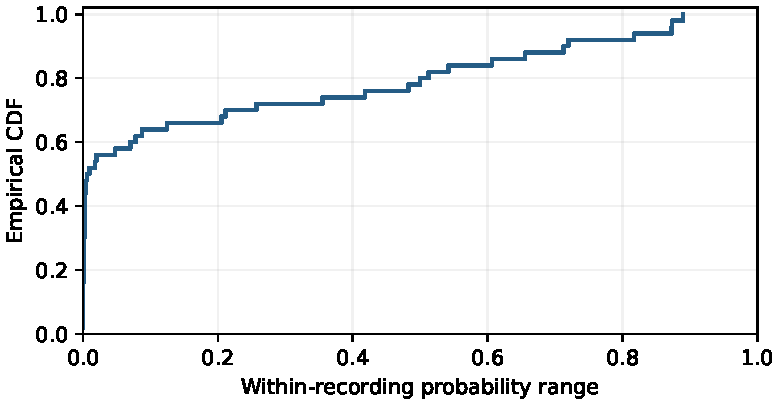
\includegraphics[width=0.66\linewidth]{figures/historical_codec_cdf.pdf}
\caption{Historical 50-recording codec experiment: probability ranges across
identity WAV and MP3/AAC/Opus variants. Mean 0.2024, median 0.0074, maximum
0.8901. The encoding helper used PCM16 staging, and some recovered inputs were
already lossy. This is a confounded audit result, not a lossless-origin,
compression-only estimate.}
\label{fig:historical-codec}
\end{figure}

The median transport range is small, but the large upper tail produces a much
higher mean (Figure~\ref{fig:historical-codec}). The result demonstrates why both
tail behavior and preprocessing identities matter. It does not establish which
part of the shift comes from quantization, encoding, prior compression, or
their interaction. The controlled experiment in the preceding section is
required to distinguish them.

\section{Completed rc2 primary comparison}

All eight checkpoints attempted all \BenchEntries{} fixed entries. Six scored
every input; ArtifactNet retained one model execution failure and native-input
DeepFense retained one input execution failure. Tables~\ref{tab:full-legacy}
and~\ref{tab:full-native} are generated from hash-verified full predictions,
using 2,000 cluster-bootstrap replicates and the fixed raw threshold 0.5.
The contemporary cohorts contain no real controls, so their TPR must be read
alongside legacy FPR rather than as a standalone accuracy ranking.

\begin{table}[ht]
\centering\small
\resizebox{\linewidth}{!}{\begin{tabular}{lrrrr}
\toprule
Detector & Scored/attempted & F1 [95\% CI] & AUROC [95\% CI] & FPR (\%) [95\% CI] \\
\midrule
ArtifactNet & 2163/2164 & 0.989 [0.985, 0.993] & 0.999 [0.998, 1.000] & 0.2 [0.0, 0.6] \\
SpecTTTra alpha-120s & 2164/2164 & 0.772 [0.755, 0.787] & 0.847 [0.832, 0.862] & 18.8 [16.3, 21.5] \\
SpecTTTra beta-5s & 2164/2164 & 0.556 [0.539, 0.576] & 0.718 [0.699, 0.736] & 11.7 [9.6, 13.9] \\
AST-60s & 2164/2164 & 0.836 [0.825, 0.848] & 0.886 [0.875, 0.898] & 26.0 [23.2, 28.9] \\
DeepFense EAT & 2163/2164 & 0.173 [0.152, 0.195] & 0.368 [0.347, 0.391] & 2.2 [1.2, 3.3] \\
Fakeprint LR (lofcz) & 2164/2164 & 0.743 [0.731, 0.756] & 0.780 [0.769, 0.791] & 12.6 [10.5, 14.9] \\
CLAM & 2164/2164 & 0.761 [0.750, 0.771] & 0.708 [0.689, 0.725] & 69.8 [66.6, 73.0] \\
FST & 2164/2164 & 0.743 [0.726, 0.759] & 0.905 [0.894, 0.916] & 1.8 [1.0, 2.8] \\
\bottomrule
\end{tabular}
}
\caption{Completed legacy comparison. Failed entries remain in attempted
coverage; metrics use available scores. Intervals are 95\% cluster-bootstrap
percentile intervals. DeepFense uses the native-input condition described below.}
\label{tab:full-legacy}
\end{table}

\begin{table}[ht]
\centering\small
\begin{tabular}{lrrrr}
\toprule
Detector & Suno scored & Suno TPR (\%) & Udio scored & Udio TPR (\%) \\
\midrule
ArtifactNet & 200/200 & 5.0 [1.9, 8.9] & 200/200 & 100.0 [100.0, 100.0] \\
SpecTTTra alpha-120s & 200/200 & 84.5 [79.4, 89.4] & 200/200 & 54.0 [47.4, 60.9] \\
SpecTTTra beta-5s & 200/200 & 42.0 [35.3, 48.5] & 200/200 & 18.0 [12.7, 23.3] \\
AST-60s & 200/200 & 99.5 [98.4, 100.0] & 200/200 & 99.5 [98.4, 100.0] \\
DeepFense EAT & 200/200 & 0.0 [0.0, 0.0] & 200/200 & 3.0 [1.0, 5.5] \\
Fakeprint LR (lofcz) & 200/200 & 100.0 [100.0, 100.0] & 200/200 & 66.5 [59.7, 72.9] \\
CLAM & 200/200 & 73.5 [66.8, 79.8] & 200/200 & 83.0 [77.2, 88.4] \\
FST & 200/200 & 54.0 [46.5, 61.5] & 200/200 & 75.5 [69.7, 81.3] \\
\bottomrule
\end{tabular}

\caption{Completed contemporary-native comparison at raw threshold 0.5.
Bracketed values are 95\% empirical cluster-bootstrap intervals; degenerate
intervals at 0 or 100\% do not establish population certainty.}
\label{tab:full-native}
\end{table}

AST detects 199/200 inputs in each native cohort, but its legacy FPR is
25.98\%; fakeprint LR detects all 200 Suno inputs with legacy FPR 12.56\%.
FST has legacy FPR 1.83\%, with Suno and Udio TPR of 54.0\% and 75.5\%.
These are observations about the evaluated checkpoints and input contracts,
not causal rankings of architectures. Provider-selected demos remain separate.

\subsection{ArtifactNet operating-point detail}

ArtifactNet has attempted all \BenchEntries{} rc2 entries, scoring 2,578 with the
same short-input execution failure retained. Table~\ref{tab:checkpoint} is
generated from its completed, hash-verified predictions and 2,000-replicate
cluster bootstrap report, providing additional operating-point detail.

\begin{table}[h]
\centering\small
\begin{tabular}{lrrrr}
\toprule
Cohort & Scored/all & TP/scored AI & TPR (\%) [95\% CI] & F1 \\
\midrule
Legacy & 2163/2164 & 1315/1343 & 97.9 [97.1, 98.7] & 0.9887 \\
Suno v5.5 (AAC) & 200/200 & 10/200 & 5.0 [1.9, 8.9] & -- \\
Udio 2026 (MP3) & 200/200 & 200/200 & 100.0 [100.0, 100.0] & -- \\
\bottomrule
\end{tabular}

\caption{ArtifactNet detail at raw threshold 0.5.
TPR intervals are empirical cluster
percentile intervals; the all-success Udio interval is degenerate and does not
establish zero population miss rate. Native F1 is undefined without real controls.}
\label{tab:checkpoint}
\end{table}

Legacy F1 is \CheckpointLegacyFone{}, whereas adding the 400 native entries
reduces non-demo mixture F1 to \CheckpointMixedFone{}. The Suno cohort's raw
TPR is \CheckpointSunoRawTpr{}\% (95\% interval
\CheckpointSunoRawLow{}--\CheckpointSunoRawHigh{}\%). The pre-existing CNN
0.225 plus rescue 0.02 stack detects \CheckpointSunoStackTpr{}\% of this cohort;
the raw-0.5 result is therefore not the only operating point showing low recall.
At raw 0.5, the provider-selected demonstrations yield
\CheckpointLyriaTP{}/\LyriaEntries{} Lyria detections and
\CheckpointStableTP{}/\StableAudioEntries{} Stable Audio detections. These tiny
demonstration counts are separate descriptive observations.

All 200 selected Suno files carry AAC audio, whereas all 200 Udio primaries are
MP3. This complete source--transport association prevents attributing their
contrast to generator version alone. The finding is poor detection under the
observed Suno source/transport conditions, not a controlled estimate of a new
generator's isolated effect. The completed controlled transport experiment helps
distinguish transport sensitivity from source differences. These results do
not change the frozen sample, thresholds, weights, or inference-failure policy.

This interpretation is consistent with a larger native-CDN audit performed
before the present benchmark. On 12,215 files, the production decision stack
(CNN threshold 0.225 plus matched rescue 0.02, codec TTA off) detected
18.49\% of Suno MP4/AAC files, compared with 90.96\% of Udio MP3 files and
50.20\% of Udio MP4/AAC files. Its historical native-pair aggregate is not used:
the numerator and percentage are inconsistent, and 156 of 1,101 shared-ID
groups contain multiple candidates without a verified recording-level join.
Reported score recovery after AAC-to-MP3 re-encoding supports transport
sensitivity, but does not establish preservation or recovery of AI-specific
information; matched real-audio controls are required. Training records identify
plain-shard CNN training and a prior augmentation assessment focused on real-side
FPR, motivating an audit of actual AI/real codec-view coverage. A July MP3
evaluation contained 1,408 Suno v5 and 802 v5.5 recordings; two earlier CNNs
detected all 802 v5.5 examples. The present comparison differs in transport,
cohort, checkpoint and evaluation conditions, so it cannot isolate their
individual effects. These historical diagnostics do not change the frozen
evaluation or its operating points.

\section{Input-path diagnostic: resampling is not neutral}

The original DeepFense adapter completed all entries, but its high legacy
false-positive rate triggered a separate compatibility diagnostic. Before
reading the diagnostic reference scores, metadata-only hash order selected
one entry from each of six legacy real-source cells, one legacy AI entry,
and one entry from each contemporary native source. These nine examples are
not a representative performance estimate, and the original run is preserved.

Fresh CPU adapter scores differed from the saved GPU scores by at most
$1.20\times10^{-7}$, with no raw-0.5 flips. Replaying the exact captured model
input gave exactly the same score on all nine examples. Keeping the common
decoded float32 44.1-kHz waveform fixed, changing only the final resampler from
TorchAudio's default to librosa's default \texttt{soxr\_hq} flipped eight of
nine decisions, with maximum absolute score shift 0.99902. All six real
examples changed from approximately 0.99 to below $3\times10^{-5}$ P(AI), but
both native AI examples also changed to real. This is not a uniformly
favorable accuracy correction.

Direct upstream SoundFile/librosa input flipped seven of eight comparable
examples; the selected Suno AAC file was unsupported by that loader and remains
an input error, not a fabricated score. The direct path changes more than the
final resampler, whereas the same-waveform control isolates that last stage.
Neither diagnostic establishes corrected full-cohort FPR or TPR. The original
DeepFense result is under an interpretation hold: it measures that adapter
condition, not intrinsic framework quality. A separately versioned, fully
evaluated input-path condition is required before the final comparison. No
checkpoint, threshold, class direction or original prediction was changed.

The implemented replacement condition, \texttt{deepfense-native-soxr/2},
decodes supported native files as float64, averages channels before direct
16-kHz \texttt{soxr\_hq} resampling, applies upstream prefix/repeat padding,
then casts to float32. It adds no clipping or common 44.1-kHz stage. An explicit
FFmpeg fallback handles only AAC or Opus rejected by SoundFile, retaining the
probed native sample rate and channel count before the same preprocessing.
This fallback is a benchmark extension, not an upstream unsupported-format
equivalence claim. Version 1's 32-source smoke produced 31 scores and one
unsupported WebM/Opus error; all original records and source snapshots remain.
Version 2 scored all 32 selected sources. The other 31 prepared waveforms,
logits and scores are bit-exact with version 1; eight comparable prior direct-
upstream waveforms and scores also match exactly. These are compatibility
checks, not representative accuracy estimates. The full 2,579-entry evaluation
completed on CPU with two threads, with this device difference explicitly
recorded: 2,578 inputs scored and one real FMA MP3 retained an input failure.
That MP3 also fails upstream SoundFile decoding; its codec is outside the fixed
AAC/Opus fallback policy, which was not expanded during evaluation.
At raw 0.5, legacy TP/FN/FP/TN are 129/1,215/18/801, with one unscored real
input: TPR is 9.60\%, FPR 2.20\%, and AUROC 0.3685. Native Suno detections
are 0/200 and Udio detections 6/200. Thus lower false positives do not establish
improved accuracy: AI detections also fall sharply. These results characterize
the measured checkpoint and input condition, not the architecture generally.
The native-input result is used in the completed eight-checkpoint comparison;
the original adapter run remains a separate audit.

\section{Controlled transport results}

For each checkpoint we scored 50 recordings under eight controlled views:
float identity, PCM16 staging, and AAC, MP3, and Opus at 128 kbps applied after
either float or PCM16 staging. The table reports mean absolute score shifts from
float identity for each lossy codec and the mean range across all eight views;
recording-cluster bootstrap intervals are available in the released JSON.
These are detector-score stability measurements, not accuracy metrics.

\begin{table}[ht]
\centering\small
\resizebox{\linewidth}{!}{\begin{tabular}{lrrrr}
\toprule
Checkpoint & 8-view range & AAC-128 & MP3-128 & Opus-128 \\
\midrule
ArtifactNet & 0.3821 & 0.0622 & 0.2229 & 0.2179 \\
DeepFense-native & 0.0729 & 0.0275 & 0.0476 & 0.0242 \\
SpecTTTra-$\alpha$ & 0.0167 & 0.0068 & 0.0040 & 0.0112 \\
SpecTTTra-$\beta$ & 0.0200 & 0.0136 & 0.0058 & 0.0059 \\
AST & 0.0374 & 0.0286 & 0.0050 & 0.0060 \\
Fakeprint LR & 0.1067 & 0.0511 & 0.0462 & 0.0526 \\
CLAM & 0.0052 & 0.0039 & 0.0006 & 0.0016 \\
FST & 0.0282 & 0.0058 & 0.0241 & 0.0027 \\
\bottomrule
\end{tabular}
}
\caption{Completed controlled transport evaluation (406 inputs per
checkpoint: 400 controlled views and 6 native-pair views). Values are mean
absolute probability shifts or the mean within-recording range. The three
native pairs are descriptive because provider transport may change more than
the codec.}
\label{tab:transport}
\end{table}

ArtifactNet is substantially more transport-sensitive than the other
checkpoints: its mean eight-view range is 0.3821, with mean MP3 and Opus shifts
of 0.2229 and 0.2179. CLAM is the most stable in this probe (0.0052 range),
while the remaining models lie between 0.0167 and 0.1067. Because the
controlled files begin from prepared benchmark audio, these estimates isolate
the declared staging and codec transformations but do not claim that the
prepared source is lossless at collection time.

\section{Reproducibility and release artifacts}

We distinguish three reproducibility checks: public metadata consistency,
statistical reconstruction from saved predictions, and fresh detector inference.
A metadata-only candidate package has passed verification after extraction into
a new directory, including six actual notebook cells. It excludes audio, model
weights, private path maps, and raw song pages. This check establishes neither
recording availability nor detector performance.

A separate local-binding command accepts user-provided file paths and checks
every primary and native-variant byte hash against the public metadata. It
emits runnable local manifests only when all required files match; unavailable
or mismatching files retain explicit audit outcomes. The original release is
not modified. Binding itself neither decodes audio nor runs a detector, and
its path-bearing output is private.

The prediction export preserves explicit failures, per-entry scores, and exact
checkpoint and source hashes while replacing absolute paths with repository-relative
identities and omitting private traceback text. A separate notebook recomputes
all eight numerical reports and 28 paired model comparisons, requiring
byte-identical statistical JSON, including the bootstrap intervals. This path
has been exercised on the actual historical smoke outputs. A public-score ZIP
containing 40 allowlisted payload files was built twice with identical hashes,
then extracted into a fresh directory. Its packaged verifier and six-cell notebook
ran from the extracted source and reproduced all nine statistical files exactly;
the existing isolated dependency environment was reused. These are software
portability checks using historical smoke scores, not full rc2 archive checks.
For full rc2, a separate results environment has now reproduced all nine
statistical files byte-for-byte from the public predictions, including all
intervals and 28 paired model comparisons. The final figure/table renderer
requires validated public predictions and exact agreement with their nine
reference statistical files. Full public admission requires the corrected
DeepFense input condition, so the original adapter audit and historical smoke
cannot enter this final rendering path. This is an implemented consistency
check that the primary result tables have passed. Saved-score reproduction
does not substitute for fresh inference with matching audio, weights,
implementations, and runtime conditions. An unauthenticated
audit of the declared public ArtifactNet repository found v9.4 ONNX exports but
none of the three exact checkpoint files required by this evaluated stack
\citep{artifactnet_public_2026}. This finding is limited to the inspected repository
revision, not all possible hosting locations. Public acquisition of the evaluated
ArtifactNet stack remains unresolved; the older ONNX model is not an equivalent
replacement. A local single-output UNet--CNN ONNX candidate now includes the
preprocessing and RMS aggregation needed for raw $P(\mathrm{AI})$, without the
LGBM rescue model. A score-blind source/boundary check covered 34 recordings:
33 had original reference scores, with maximum absolute difference
$5.09\times10^{-4}$ and no raw-0.5 decision flips; the original failed recording
remained non-comparable. The predeclared rule is absolute difference at most
$10^{-3}$ and zero such flips. A fresh execution without PyTorch reproduced one
candidate score exactly. These are engineering checks, not full rc2 parity or
evidence of public model availability. During full verification, one of the
first 205 comparisons exceeded the fixed tolerance: $0.729230$ on the original
GPU versus $0.728190$ in ONNX CPU, a difference of $1.0404\times10^{-3}$.
A targeted same-input diagnostic gave $0.728272$ for the original CPU
implementation. Substituting native FFT STFT in the PyTorch export graph
reproduced that CPU score within $2.3\times10^{-16}$, while the DFT-convolution
graph gave $0.728190$. This separates a larger saved-GPU/fresh-CPU discrepancy
from an additional STFT-path contribution on this recording; it is not a
population result or justification for relaxing the predeclared tolerance.
The original full verification was interrupted by a system reboot and remains
incomplete, without a full-parity success claim. Model publication and the additional rescue-stack reproduction
path remain unresolved.

The manuscript is maintained as LaTeX source. Final tables and figures are to be
generated directly from the completed, hash-bound reports, with provider-selected
demonstrations kept separate. The submission source archive must include the
bibliography and generated figures and tables, but not private inputs. This
draft is not evidence of publication or an arXiv submission.

\section{Limitations, rights, and responsible interpretation}

The sampling frame is a collection of accessible recordings, not a probability
sample of all published music. Creator caps reduce domination by prolific
accounts but cannot remove popularity, genre, language, availability, or
provider-selection bias. Handles can change, creator metadata can be incomplete,
and dependencies between remixes may not be fully disclosed. External detector
training manifests can be unavailable. Every one of these limits constrains
generalization claims even after identified duplicates have been grouped.

Platform-generated-or-edited recordings include hybrid workflows. A detector
score cannot establish authorship, copyright ownership, permission, or intent.
False accusations can harm musicians, particularly in contexts with low AI
prevalence. The benchmark measures acoustic classification under declared
labels; it does not provide a sufficient basis for automatic punitive decisions.

Public playback does not establish redistribution permission. The release
therefore separates public metadata and reconstruction instructions from local
audio and audit snapshots. Dataset and model licenses are source-specific.
Official demos remain separately labelled, and unavailable recordings remain
visible through access outcomes and hashes. No commercial model access terms
are accepted or paid generation initiated merely to fill a quota.

\section{Conclusion and completion requirements}

ArtifactBench 1.2 treats provenance and coverage as parts of an evaluation,
not optional annotations. The historical audit establishes concrete reasons
for version-evidenced sampling, full-file validation, separate operating stacks,
and controlled transport tests. The release-candidate data are frozen, and the
eight-checkpoint primary comparison exposes substantial source-dependent detection
and false-positive trade-offs under confounded source/transport conditions.
Its public-score statistics reproduce exactly, and the controlled transport
evaluation is complete. Full release portability and model-release verification
remain required.
Until these are complete, this document remains a draft, not a
completed benchmark release or a submission-ready paper.

\bibliographystyle{plainnat}
\bibliography{refs}
\end{document}
